Several concepts are necessary to understand the context for the major technical accomplishments of this independent study. One of the most important ones is the most important is the difference between local and global space. Blender stores an object's cartesian coordinates, scale, and rotation in two separate matrices: local and global. The global matrix represents an objects position and orientation with respect to a fixed center shared by all objects in a scene. The local matrix represents position and orientation with respect to another coordinate system centered at the initial center of the object. The two are disjoint and separate: altering one will not affect the other. It is important to note this difference, because many built-in functions and variables in blender (such as the coordinates of vertices and the return values for some ray-casting functions) will return local and not global vertices. Figure XX below illustrates the difference between local and global coordinates ([1]).

\begin{wrapfigure}{r}{0.5\textwidth}
	\begin{center}
		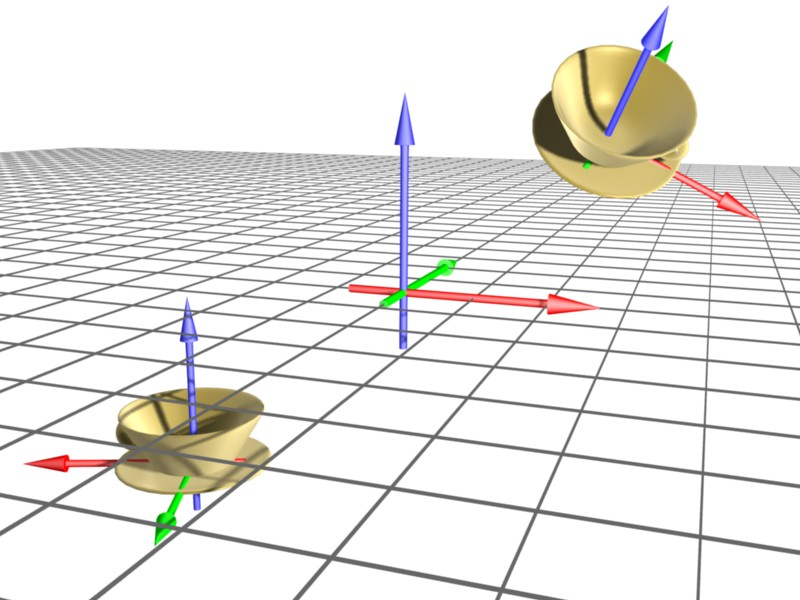
\includegraphics[width=0.48\textwidth]{figures/3dspace.jpg}
	\end{center}
	\caption{Human and AI agents have similar move optimality across all tests.}
\end{wrapfigure}

The difference between the two has caused a number of problems with the project, particularly because certain functions return coordinates in one space, and others return it in the other. Although it is possible to convert local to global and vice-versa, these differences are not usually documented, and can complicate debugging considerably.

Another important concept is that of ray-casting. Ray-casting is a technique for tracing a line from one point to another in a 3D environment ([8]). The exact algorithm begins by tracing pixels from the start end of the cast to the end, and as such can very easily be used for line of sight and distance calculations. Blender has a number of ways of implementing ray-casting, and the decision of which to use in which context influenced code design heavily.

Blender only contained a ray-casting method which was a method in the Object class. This means that any ray-casting had to be called from a given object, even when no object was necessary for the casting. It also returned the coordinates of the end destination (if an object was hit by the cast) in local coordinates, rather than global. However, with the newly release blender version 2.68, the Scene class came equipped with a similarly functional ray-casting function. This method operated in global space, and as such was much preffered to the former. A separate copy of the Blender executable was carried with the project files until recently, when the school's computer system upgraded its version of blender.

Several changes new functions were added to the obutils.py module. First among them was deleteObject and deleteAllObjects. The purpose of these should be intuitive: the former delted a single, specified blender mesh object from the scene. The latter deleted all blender mesh objects from the scene (with the exception of the standard lamp and camera object). A nudge and cast\_thru function were also added, as well as a custom rayCast function. All three were utilized by the vision predication, and the latter is a wrapper for the scene ray cast discussed above. RayCast allowed the user to use the scene ray cast without having to pass the scene as a parameter. This was doable since all of our experiments took place in only one scene. Cast\_thru and nudge's uses are more specific, and are discussed in detail further on.

Our project began with a working, though rudimentary, implementation of basic placement and querying methods. Several experiments were run at the beginning of the semester, and the IRS demonstrated the ability to place certain objects and certain predicates with reasonable accuracy. These algorithms, however, were exceedingly simple, and were not accurate enough for the purposes of the project.
To begin with, the “near” predication was not sufficiently generalized to deal with objects disproportionately sized in one dimension. The old method of querying near(A,B) involved taking the largest of the set of the union of A and B's dimensional measurements, and calculating whether or not the distance between the center points of the two objects was within that boundary. If it was, then the query method returned one. If it was greater than this, then the return value was calculated by an exponential function 

\begin{center}
$y = 2e^{-.6931(x-D)}$
\end{center}

Where y is the value returned and D is the aforementioned maximum dimension between the two entities. However, this did not match well with the semantic interpretations of the predication.
First, an entity is considered to be “near” another if the two have a point in space in their objects that is proximate, and the proximity of their center points is irrelevant. For example, an individual can be right next to a city (though two miles from its center) and still be considered “near” it. For this reason, the code was changed to utilize the BPY closest\_point\_on\_mesh function, which returned the closest point between two mesh objects. This allowed the code's answers to more accurately represent the predication.
Second, the methods did not account for object which were significantly longer than they were wide or tall. Objects such as walls, fences, and rivers (informally called “arbitrarily large”) were not handled correctly by the code. In the old implementation, the code would select the largest dimension of the object, in this case, the length, and use that as the heuristic to determine nearness. This would mean that an individual would be considered “near” a small fence if he was within several hundred meters of it, which is of course absurd. 
To remedy this, an added function was programmed into obutils.py. This function, isAbritrarilyLarge(A), took a given object iterated through its dimensions. If one dimension was more than 100 times larger than the others, then the function returned true. If this occured, the object would use as a heuristic the square root of the sum of the squares of the two remaining dimenisons.
By far, however, the largest and most complicated predicated added over the course of the study was the canSee(A,B) predication. This held if entity A was capable of seeing entity B. The implementation of this function relied heavily on ray-casting (see above) and went through several iterations before a sufficient model and algorithm was developed. 
The querying method for this predication originally was to be implemented as a single ray-cast, from one object's center to another. Over the summer, a number of different attempts to construct a sufficient canSee(A,B) function were tested, yet none were of the quality needed for the project. Examples include the use of a conical object expanding from entity A's “eye” to B and noting the percent of B's volume that was encompassed inside, and several functions in Blender's Game Engine. At the beginning of the study, a function existed which ray-casted from the center-point of A to the center point of B. This function was naiively simply, but proved itself to be suprisingly difficult to implement. For a graphical representation, Figure XX below illustrates the ideal for this model.

\begin{figure}{r}
	\begin{center}
		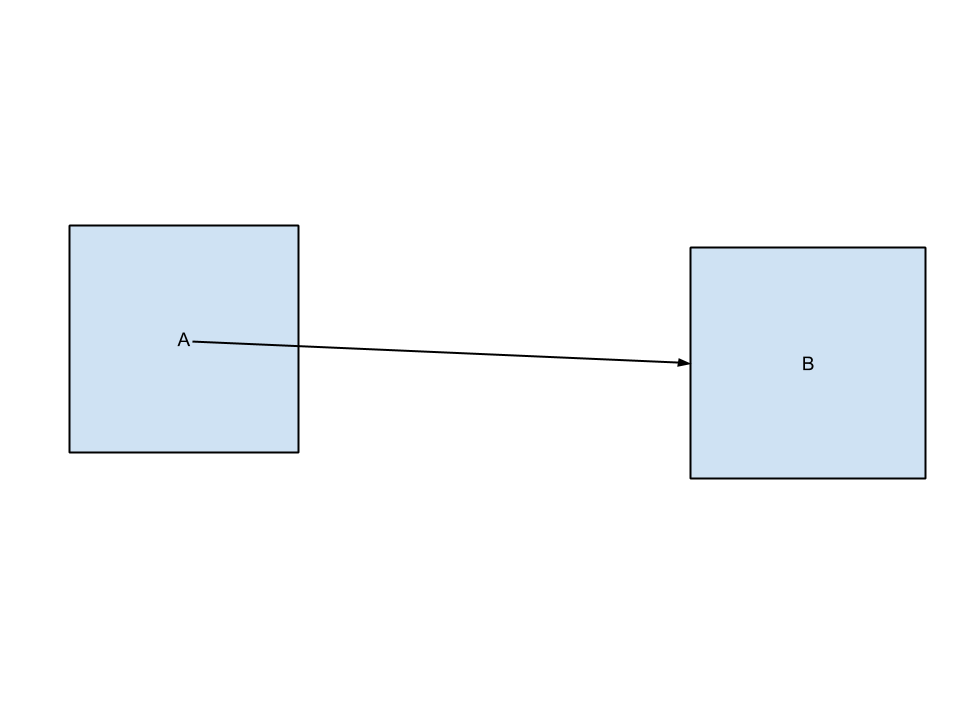
\includegraphics[width=0.48\textwidth]{figures/vision1.png}
	\end{center}
	\caption{An idealized model of the naive implementations}
\end{figure}

One issue that came up with this design was the collision nature of ray-casting. Namely, a given ray-cast in blender will return when it hits an object, any object. This means that casts from A's center would always stop upon hitting A's outer mesh. One early attempt to solve this was to simply implement repeated casting: the method would cast continuous rays from the end of one to the start of the other until the end object was met. Figure XX shows the idealized version of the function of this implementation of the function.

\begin{figure}{r}
	\begin{center}
		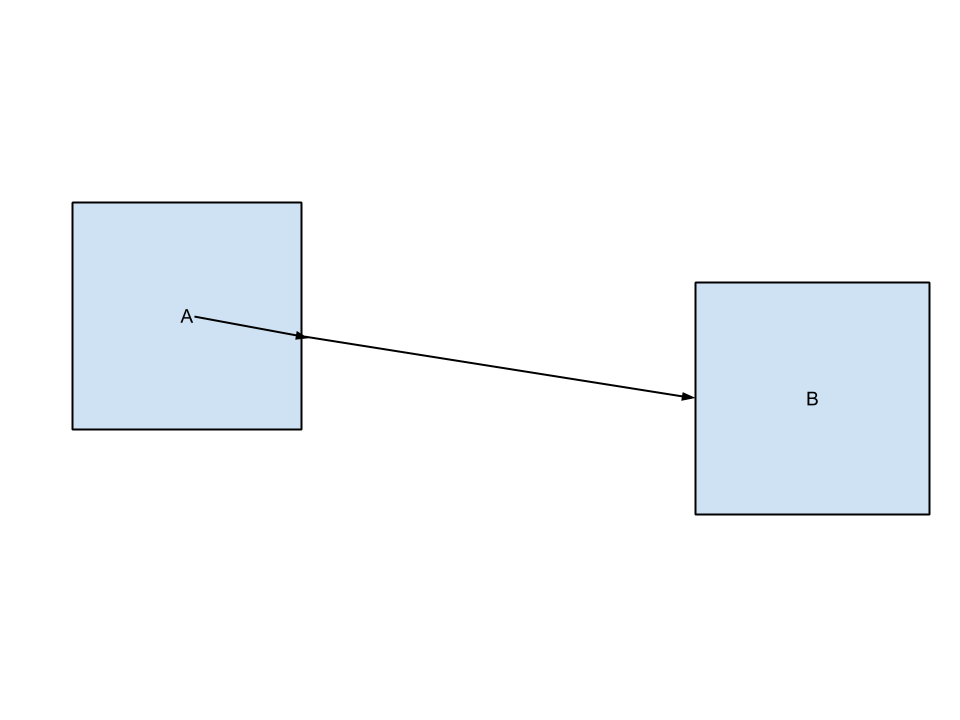
\includegraphics[width=0.48\textwidth]{figures/vision2.png}
	\end{center}
	\caption{A second implementation of ray-casting}
\end{figure}

This revealed yet another problem, however, as casting from the face of one object (which was the collision point of the fist ray-cast in the above) would simply return the starting point of the cast. The ray-cast could repeat infinite times and still be stuck on the same point! The third iteration of this function was meant to take care of this. This iteration involved the addition of another method in obutils.py, nudge(pt\_a,pt\_b) which would return an infinitesimally small distance closer to the end point. This function allowed repeated ray-casting to continue unabated and as planned. The new model for ray-casting in this simple iteration is illustrated in figure XX. 

\begin{figure}{r}
	\begin{center}
		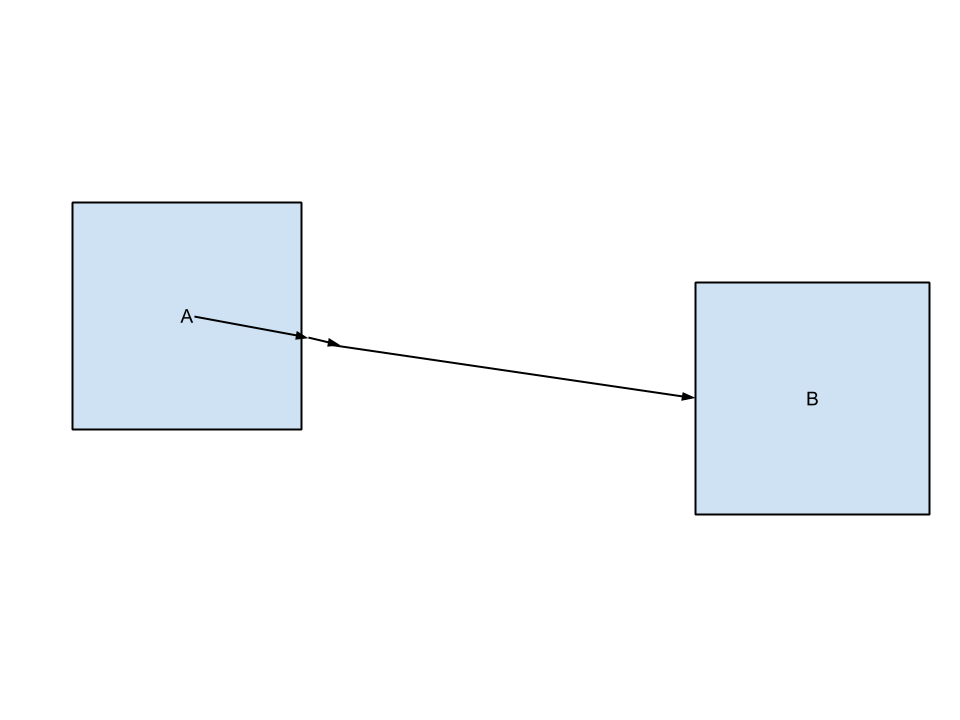
\includegraphics[width=0.48\textwidth]{figures/vision3.png}
	\end{center}
	\caption{the nudge addition to the naive model}
\end{figure}

This model was able to accurately cast a ray from the center of A to B, stopping when it hit B's outer mesh. However, the naive model was, as the name should suggest, not sufficient and could easily return erroneous answers. For example, if there was an object in between A and B which could block the cast, then the method would conclude that A could not see B, even if it were obvious that a line of sight existed between the two. Figure XX illustrates this.

\begin{figure}{r}
	\begin{center}
		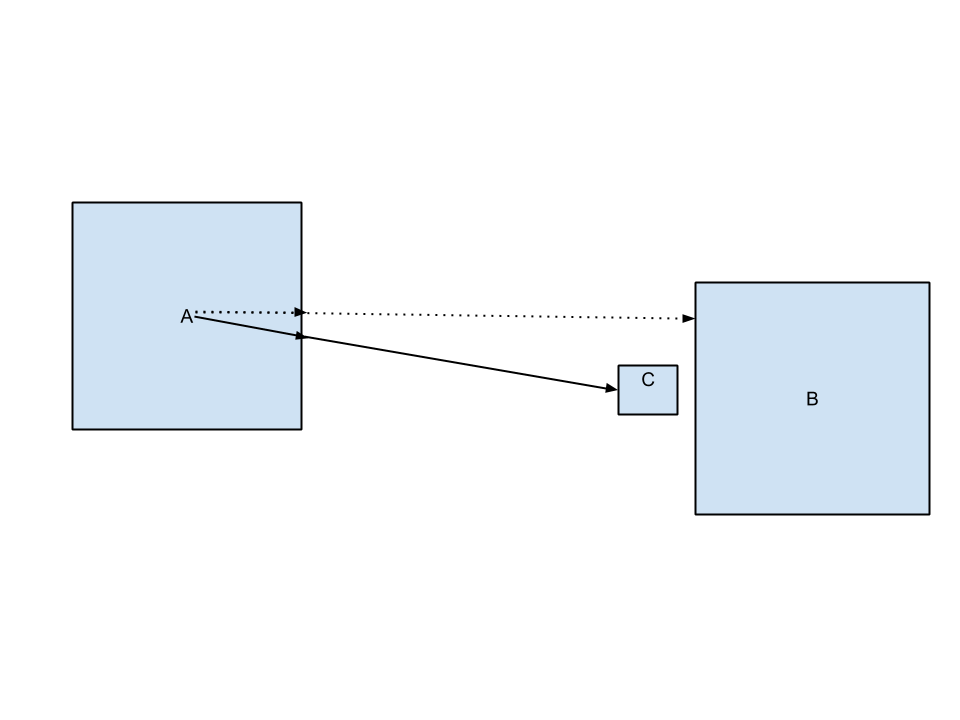
\includegraphics[width=0.48\textwidth]{figures/vision4.png}
	\end{center}
	\caption{C blocks the site of A, even though there exist obvious casts (dotted) that would indicate that B is visible}
\end{figure}

It was obvious early on that this implementation would only serve as a template for future endeavors.
The second model used cast a slew of rays from A to the vertices of B. This improved over the naive implementation in two ways. First, it allowed a varying degrees of visibility. Several of the rays may reach their target, and several may not, which allowed for a sense of “partial obscurity” which was not allowed in the original model. This ran into a small technical issue early on, however, as rays would not return if they made contact with the vertices of an object. Due to a technicality in blender, casts would only return if they made contact with the face of an object. As such, a modification of the nudge function was implemented which pushed the end point of the casts closer to the center. This way, there was a guarantee that the casts, if unobstructed, would hit the object properly. Figure XX illustrates this model.

\begin{figure}{r}
	\begin{center}
		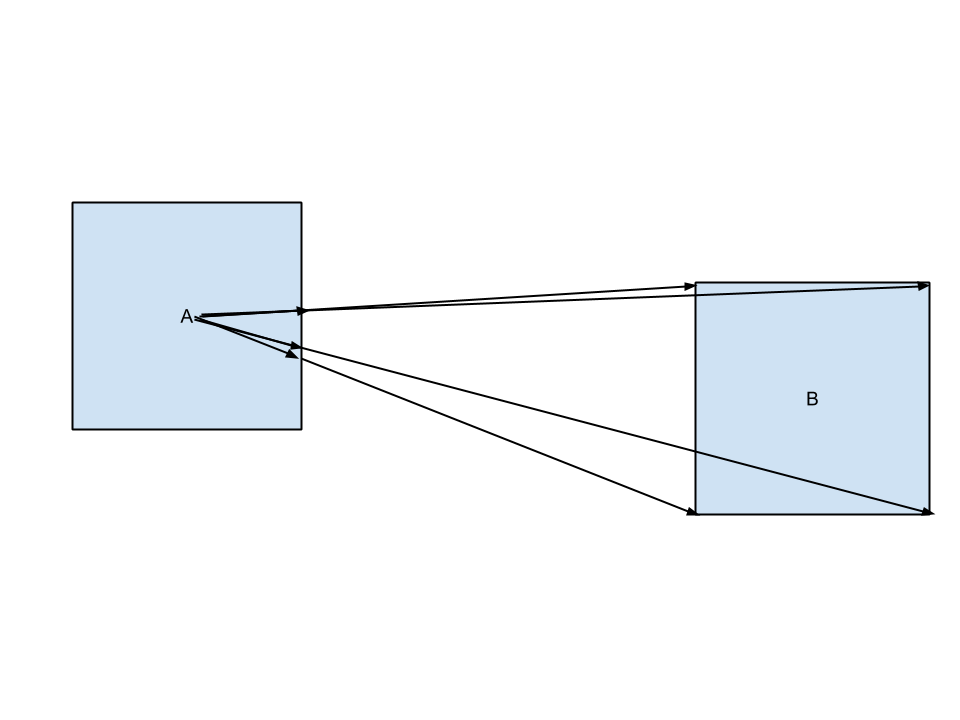
\includegraphics[width=0.48\textwidth]{figures/vision5.png}
	\end{center}
	\caption{Figure XX: the second iteration of the canSee(A,B) algorithm}
\end{figure}

This model was not perfect, however, in that it could give bias to an object if there were a large number of vertices concentrated at a given section of the object. In Figure XX, we show how this coulud be problematic. A would cast a disproportionate amount of rays to B's bottom side, which would collide with C, giving the impression that B is much less visible than it actually is.

\begin{figure}{r}
	\begin{center}
		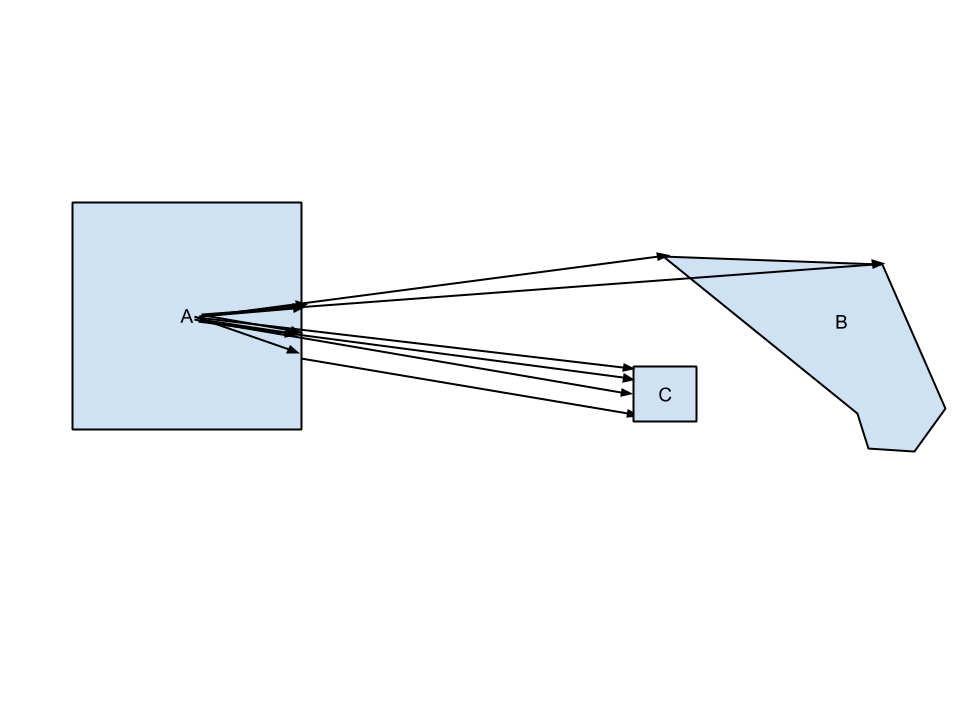
\includegraphics[width=0.48\textwidth]{figures/vision6.png}
	\end{center}
	\caption{The majority of the casts are blocked by C even though B is visible}
\end{figure}

One suggested solution to this situation involved weighting the vertices depending on how close they were. In this interpretation, casts to close-by vertices would be “worth less.” If these successfully hit their target, they would return a number less than one. The exact waiting system was not decided. This system, however, proved to be unnecessary, as the final algorithm removed the need for vertices entirely. 

The final system utilized an obscure library in Blender Python (BPY\_extras) to grasp random points on the meshes faces. Rays were cast to these points, and the percent of casts that returned were used to evaluate the visibility of the target object. This method was both fair and correct. The number of rays cast to a given face was proportional to the face's percent of the total surface area of the object, which ensured that the most visible (largest) faces would receive the most casts. Because the number of samples is proportional to the size of the object's faces, no section of the object will overrepresent itself in testing. Figure XX shows how the new method solves the problems of the old.

\begin{figure}{r}
	\begin{center}
	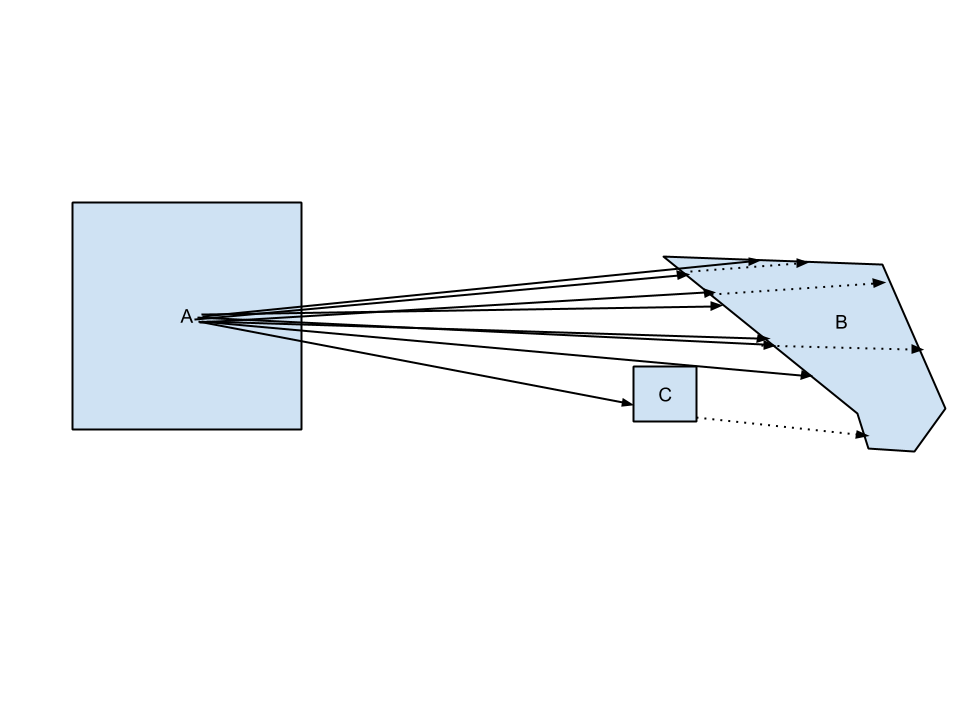
\includegraphics[width=0.48\textwidth]{figures/vision7.png}
	\end{center}
	\caption{Rays are cast evenly across object B}
\end{figure}

The final change to the vision predication involved compensation for opacity. It was desired that the visibility of an entity not simply depend on line of sight, but also on the presence of partially occluding object en route to the object. This was solved through custom properties and repeated casting. Each ray-cast was given an initial value of 1. The cast traveled through space as in the above model. When another object was encountered, the behavior of the cast differed depending on the object hit. If the object was the target object, then the cast returned it's value (initially set to one). If it encountered a different object with no occlusion property (or occlusion of one) then the hit object was assumed to be completely opaque and the cast returned zero. If the object hit an object with an occlusion value between zero and one, then the object recast towards its target, but the value of the occlusion property was added to an “occlusion counter” for the cast. This occlusion counter would would be reduced by the occlusion amount of the object when the cast left the object.
As the cast traveled through an object, the value would degrade proportional to the current counter. If the return value was reduced to zero, then the cast would fail and the function would return zero. Thus, the further through an obscuring object (such as a fog or the leaves of a tree) an object was, the more obscured it became. The “occlusion counter” was necessary in order to allow multiple obscuring factors affect the object. This corresponds to situations such as man looking at a bird through a tree in a fog.
This change in paradigm necessitated the introduction of a new function in obutils.py: cast\_thru. This function performed all of the above functions, and took care of the repeated casting (including calls to ray\_cast and nudge). The initial cast was handled by the predicateMethods.py file, and subsequent casts were all done in the cast\_thru module. This led canSee to a slightly different larger dependence on obutils.py functions than other predications.

The largest change to the system over the course of this study has, however, been the adjustment of the predication and associated methods to adhere to the new object paradigm. Up until this semester, the predication only worked for single Blender mesh objects. This was done for object testing purposes. The simplified objects allowed for adequate testing of the parameters of the predications. The actual objects (“entities”) in the system, however, are not mesh objects. Entities are data structures consisting of a list of mesh objects which are children to a point “parent” object. In order to make the adjustment to fit this paradigm, significant changes were necessary in the code. A standard methodology was adopted for passing objects and entities as parameters. All obutils.py functions were assumed to take blender mesh objects as parameters. Although some functions exist which could take entities as well, for the sake of simplicity it was simply assumed that all obutils.py methods only took objects. 
Predication functions (in predMethods.py), however, always too entities. Because these methods were supposed to operate at the high level of abstraction utilized by the Classes module, it made more sense to requires the use of entities in these methods. This is in contrast to the functions in obutils.py, which were meant to interface directly with Blender objects and, as such needed to operate on a lower level of abstraction. The outline of this can be seen in figure XX in the previous section.
GetVolume was the first function to be altered. Because this function was adopted from a function issued by the GNU project, the internal workings of the code were not altered. A wrapper method was simply utilized which determined whether or not the parameter passed was an entity (i.e. whether or not it had children) and, if it did, ran the getVolume function on all of its children, returning the aggregate volume of the set. If no children were found, then the parameter was assumed to be a Blender object, and only the volume of the parameter itself was returned.
Deleting objects similarly utilizes a wrapper tester. Both functions were able to be utilize both parent and child objects. One of the properties of Blender's object hierarchy is the dependency of child objects to parent ones. If the parent is deleted, all children are as well. Therefore, it mattered little whether an object had children, if a parent was passed, it was deleted as well!
Conversely, the duplicateObject method was unable to be coerced to take parent objects. Although there are relationships between parent and child objects, the former do not have meshes, and they are both distinct objects with. This means that attempting to duplicate an object would involve separate code for duplicating the parent and child objects, as well as joining them so that they have the same structure as the original object. 
This was avoided for two reasons. First, these methods were not necessary for this function. The  duplication function it only used to recreate meshes so that intersections between small mesh objects can be calculated, there is little purpose to duplicating a full sized object. Second, this level of complexity brings the function very close to the object creation methods in the Classes.py module, which make duplication of this kind redundant.
The loc\_by\_vert function was added to allow the computation of location of child objects. This was required because in our implementation child objects share their location (in global coordinates) with their parent object, and this gave an inaccurate representation of their position for obvious reasons.
MaxDim was altered to take the accumulation of all vertices in all children if a parent object was passed, and to run the original code if a child object was passed as a parameter. Similarly, closestPoints iterated either through one object or all child objects depending on the nature of the object passed.
Many attempts were made to get getDiff and getIntersection to function with parent objects. However, the process by which the interesection and difference operators work is very tempermental. If there are any breaks in any meshes (unclosed faces, out of place vertices, etc) the function will fail. Because the parent objects of children to not share meshes, reworking these methods to take parent objects was not feasible.
Lowest and highest point functions were able to take either parent or child objects, the difference between the two was simply the addition of another level of iteration to grab all the vertices of all the children (as opposed to all the vertices of just one object). AlignMeasure was one of the easiest functions to modify, the only change needed was to specify the location of the measure-cube with loc\_by\_vert rather than the built in location if a child object was passed. IsArbitrarilyLarge was also fixed simply by adding an additional layer of iteration if a parent object was passed. All other functions not mentioned did not require alterations in order to fit with the new object paradigm.
Although much of the incompatability was caused by utilized methods in obutils.py, many of the methods in predMethods.py also required modification in order to function properly. Under(A,B)'s query function requied the addition of an iteration through child objects in order to adequately evaluate the predication. For each child in B, a measure-cube was constructed underneath A, and the column of the intersection was noted. The aggregate volume of all intersections was compared with the total volume of B to determine the volume of B.
Similar methods were deployed for in(A,B), inside(A,B), and above(A,B). All involved iterating through the children and comparing the volume of each that was within the specified measure-cube. canSee(A,B) was slightly more complicated. Originally, the query method simply casted rays to an object's faces depending on each's proportion of the total surface area. However, this was problematic for the new model. With multiple children, the percent surface area of each face sometimes dipped below one percent, and one cannot do “half a ray-cast.” Thus, in the new method, the faces of all child object were sorted according to surface area. Starting with the face with the highest surface area, rays were cast proportional to the total surface area (at minimum one) until the total amount of rays to be cast was exhausted. This system still prioritized larger faces in a fair manner (never giving preference to certain parts of the target object over others), but also dealt with the situation where an object is made of many very small faces effectively.
Our placement functions were much more easily converted than the querying methods. Because our placement methods were generally very rudimentary (utilizing heuristics to build a “rectangular prism” representing potential placement points) there was little work that needed to be done in order to successfully place the objects.
In addition to technical improvements, a number of netowrking accomplishments were made this semester. One of this year's Cornell Cup teams, Haptek, planned to use haptic feedback gloves in order to create a virtual maze. The group's project was to have an individual wearing sensors on their head, arms, and torso stand in a room monitored by motion-sensitive cameras. The cameras would project the individual's frame into a virtual maze, and would alter their position in the virtual maze corresponding to their real position in the room. The virtual environment would also contain wall objects, and when the user's virtual image collided with a virtual wall, the persons sensors would vibrate. Through this method, the individual would be able to navigate a virtual maze as though they were immersed inside it.
After contacting Dr. Thaddeus Pawlicki about a potential collaboration, it became apparent that the IRS could serve as the program to host the virtual environment. The 3D simulation and predicate querying necessary for commonsense reasoning in 3D is precisely the system needed for this particular endeavor. The haptek virtual environment would essentially contain several entities (one of which was a human) which would receive updates from the environment (in this case, not symbolic logic and relationships but explicit position updates). The system would, after each update, query the user entity to examine if it was touching (or inside) any of the wall entities. The alterations to the code are already underway, and analysis and testing of the system will begin when the hardware components of the project are finalized.
Second, I was able to contact Dr. Benjamin Johnston for advice and potential collaboration on with our project. Dr. Johnston's dissertation on his Comirit project is a major influence and motivation for this project. Comirit is high level abstraction and framework which has shown success in its ability to utilize 3D simultion to solve commonsense reasoning problems ([CITE]). Dr, Johnston has also expanded his project to include means for implementing voxel-based objects, and has created a website for crowd-sourced development of these constructions ([CITE], [CITE]). Collaboration was worth looking into with Dr. Johnston because the IRS project was (and is) currently looking for more efficient means of creating entities and objects for our object database. Although we did receive a response and were able to establish a correspondence with Dr. Johnston, his crowd-sourcing project had been a short-lived endeavor, accumulating only 20 objects.
